\documentclass{ximera}

\newcommand{\dfn}{\textbf}
\renewcommand{\vec}[1]{{\overset{\boldsymbol{\rightharpoonup}}{\mathbf{#1}}}\hspace{0in}}
%% Simple horiz vectors
\renewcommand{\vector}[1]{\left\langle #1\right\rangle}
\newcommand{\arrowvec}[1]{{\overset{\rightharpoonup}{#1}}}
\newcommand{\R}{\mathbb{R}}
\newcommand{\transpose}{\intercal}
\newcommand{\ro}{\texttt{R}}%% row operation
\newcommand{\dotp}{\bullet}%% dot product

\usetikzlibrary{calc,bending}
\tikzset{>=stealth}


\usepackage{mdframed} % For framing content
%\usepackage{ifthen}   % For conditional statements

% Define the 'concept' environment with an optional header
\newenvironment{concept}[1][]{%
  \begin{mdframed}[linecolor=black, linewidth=2pt, innertopmargin=5pt, innerbottommargin=5pt, skipabove=12pt, skipbelow=12pt]%
    \noindent\large\textbf{#1}\normalsize%
}{%
  \end{mdframed}%
}











%% \colorlet{textColor}{black}
%% \colorlet{background}{white}
%% \colorlet{penColor}{blue!50!black} % Color of a curve in a plot
%% \colorlet{penColor2}{red!50!black}% Color of a curve in a plot
%% \colorlet{penColor3}{red!50!blue} % Color of a curve in a plot
%% \colorlet{penColor4}{green!50!black} % Color of a curve in a plot
%% \colorlet{penColor5}{orange!80!black} % Color of a curve in a plot
%% \colorlet{penColor6}{yellow!70!black} % Color of a curve in a plot
%% \colorlet{fill1}{penColor!20} % Color of fill in a plot
%% \colorlet{fill2}{penColor2!20} % Color of fill in a plot
%% \colorlet{fillp}{fill1} % Color of positive area
%% \colorlet{filln}{penColor2!20} % Color of negative area
%% \colorlet{fill3}{penColor3!20} % Fill
%% \colorlet{fill4}{penColor4!20} % Fill
%% \colorlet{fill5}{penColor5!20} % Fill
%% \colorlet{gridColor}{gray!50} % Color of grid in a plot


\author{Parisa Fatheddin \and Tae Eun Kim \and Bart Snapp}


%% https://ghenshaw-work.medium.com/3-ways-to-understand-matrix-multiplication-fe8a007d7b26


\title{Matrices, products, and equations}


\begin{document}
\begin{abstract}
  A concrete introduction to matrices and their connections to systems
  of equations.
\end{abstract}
\maketitle

\begin{quote}
  Probably no other area of mathematics has been applied in such
  numerous and diverse contexts as the theory of matrices. In
  mechanics, electromagnetics, statistics, economics, operations
  research, the social sciences, and so on, the list of applications
  seems endless. By and large this is due to the utility of matrix
  structure and methodology in conceptualizing sometimes complicated
  relationships and in the orderly processing of otherwise tedious
  algebraic calculations and numerical manipulations.



  \hfill ---\link[J.\ Cochran]{https://go.osu.edu/cochran}
\end{quote}




A \dfn{matrix} is just a large rectangular array of numbers
\[
M =
\underset{\displaystyle\boldsymbol{5}~\textbf{columns}}{\begin{pmatrix}
  a_{1,1} & a_{1,2} & a_{1,3} & a_{1,4} & a_{1,5} \\
  a_{2,1} & a_{2,2} & a_{2,3} & a_{2,4} & a_{2,5} \\
  a_{3,1} & a_{3,2} & a_{3,3} & a_{1,4} & a_{3,5} \\
  a_{4,1} & a_{4,2} & a_{4,3} & a_{4,4} & a_{4,5}
\end{pmatrix}}
~~\boldsymbol{4}~\textbf{rows}
\]
We give the \dfn{dimensions of a matrix} by stating its number of rows
and number of columns. The number of rows comes first and the number
of columns second, so $M$ above is a $(4\times 5)$-matrix.
\begin{question}
  Which of the following matrices are $3\times 2$ matrices?
  \begin{selectAll}
    \pdfOnly{\begin{multicols}{4}}
  \choice{$\begin{pmatrix}
  2 & 4 & 8\\
  5 & 9 & -1\\
  6 & 0 & 1
    \end{pmatrix}$}
  \choice{$\begin{pmatrix}
  0 & 1 &3\\
  0 & 0 & 2
  \end{pmatrix}$}
  \choice[correct]{$\begin{pmatrix}
  2 & 1 \\
  4 & 5 \\
  -1 & 0
  \end{pmatrix}$}
  \choice[correct]{$\begin{pmatrix}
  0 & 0\\
  0 & 0 \\
  0 & 0
    \end{pmatrix}$}
  \pdfOnly{\end{multicols}}
  \end{selectAll}
\end{question}


We can use similar notation to talk about specific entries of a
matrix. Above, $a_{i,j}$ is the $\boldsymbol{(i,j)}${\bf-}\dfn{entry}
of the matrix $M$ (we usually use capital letters for matrices). Often
people write $M_{i,j}$ (or just $M_{ij}$) to mean the $(i,j)$-entry of
the matrix $M$.



\begin{question}
  If
  \[A= \begin{pmatrix}
  -3 & 0 & 1\\
  4 & 5 & -2\\
  0 & 9 & -1
  \end{pmatrix}
  \]
  what are the entries $A_{1,2}$, $A_{2,2}$, $A_{3,2}$?
  \begin{prompt}
    \[
    A_{1,2} = \answer{0}, \quad A_{2,2} = \answer{5}, \quad A_{3,2} = \answer{9}
    \]
  \end{prompt}
\end{question}

Next we'll discuss how matrices arise in different contexts.


\section{Matrices store data}


A matrix can be thought of as a ``mathematical spreadsheet.'' With a
spreadsheet you have rows and columns of data.  The data we're
typically interested in comes in the form of vectors.  You can think
of a matrix as vectors stacked together either horizontally or
vertically.

\begin{example}[Population Counts] %https://worldpopulationreview.com/states/states-by-race
  In a previous example, we encoded the $2023$
  \link[demographics]{https://worldpopulationreview.com/states/states-by-race}~of
  the twelve Midwestern States as $6$-dimensional vectors represented
  as ordered tuples. Represent this data by a $12\times 6$
  matrix. Explain what the entry at position $(7,5)$ represents.
  \begin{explanation}
  Since ordered-tuples are \wordChoice{\choice[correct]{horizontal}\choice{vertical}} it makes sense to
  concatenate this data by stacking it horizontally into a matrix:
  \[
  \begin{pmatrix}
  \vec{p}_{\texttt{IA}} \\
  \vec{p}_{\texttt{IL}} \\
  \vec{p}_{\texttt{IN}} \\
  \vec{p}_{\texttt{KA}} \\
  \vec{p}_{\texttt{MI}} \\
  \vec{p}_{\texttt{MN}} \\
  \vec{p}_{\texttt{MO}} \\
  \vec{p}_{\texttt{ND}} \\
  \vec{p}_{\texttt{NE}} \\
  \vec{p}_{\texttt{OH}} \\
  \vec{p}_{\texttt{SD}} \\
  \vec{p}_{\texttt{WI}}
  \end{pmatrix}
  =
  \begin{pmatrix}
  2806418 & 117035 & 10538 & 79296 & 3941 & 132783\\
  8874067 & 1796660 & 33972 & 709567 & 5196 & 1296702\\
  5510354 & 631923 & 14030 & 158705 & 2205 & 379676\\
  2416165 & 165837 & 22278 & 87093 & 2344 & 218902\\
  7735902 & 1360149 & 50035 & 316844 & 3117 & 507860\\
  4572149 & 359817 & 54558 & 275242 & 2201 & 336199\\
  4978046 & 698043 & 24274 & 123810 & 8887 & 291100\\
  651470 & 23959 & 39165 & 11979 & 1004 & 32817\\
  1641256 & 91896 & 16875 & 47944 & 1235 & 124620\\
  9394878 & 1442655 & 20442 & 268527 & 3907 & 544866\\
  735228 & 18836 & 74975 & 12413 & 544 & 37340\\
  4895065 & 367889 & 48674 & 163396 & 2672 & 329279
  \end{pmatrix}
  \]
  Note that the above is a $\answer[given]{12}\times \answer[given]{6}$ matrix. The $(7, 5)$-entry is
  $\answer[given]{8887}$ which is the number of Hawaiians in Missouri (MO).
  \end{explanation}
\end{example}





\begin{example}[Grayscale Image]
  Here is a very low resolution grayscale image of the number $6$:
  \begin{center}
\newcommand{\matrixData}{{
    {0, 0.01, 0, 0, 0, 0, 0},
    {0, 0, 0.06, 0.18, 0.18, 0.01, 0},
    {0, 0.38, 0.64, 0.21, 0.37, 0.79, 0.06},
    {0.12, 0.99, 0.12, 0.01, 0, 0.11, 0.02},
    {0.34, 0.94, 0.32, 0.41, 0.64, 0.55, 0.02},
    {0.35, 0.97, 0.09, 0, 0.05, 0.98, 0.43},
    {0.14, 0.98, 0.13, 0, 0.01, 0.94, 0.39},
    {0, 0.34, 0.56, 0.29, 0.47, 0.51, 0.01},
    {0, 0, 0, 0.07, 0.03, 0, 0},
    {0, 0.01, 0, 0, 0, 0.02, 0}
}}
    \begin{tikzpicture}[scale=.5]
      \foreach \y in {1, ..., 8} {
        \foreach \x in {0, 1, ..., 6} {
          \pgfmathsetmacro\val{\matrixData[\y][\x]}
          \fill[black, opacity=\val] (\x, -\y) rectangle (\x+1, -\y-1);
          \draw (\x, -\y) rectangle (\x+1, -\y-1);
        }
      }
    \end{tikzpicture}
  \end{center}
  We can represent this data as an $8\times 7$ matrix where $0$
  represents ``black,'' $1$ represents ``white,'' and numbers in between represent ``shades of gray.''
  \[
  \begin{pmatrix}
     1 & 1 & 0.94 & 0.82 & 0.82 & 0.99 & 1 \\
     1 & 0.62 & 0.36 & 0.79 & 0.63 & 0.21 & 0.94 \\
     0.88 & 0.01 & 0.88 & 0.99 & 1 & 0.89 & 0.98 \\
     0.66 & 0.06 & 0.68 & 0.59 & 0.36 & 0.45 & 0.98 \\
     0.65 & 0.03 & 0.91 & 1 & 0.95 & 0.02 & 0.57 \\
     0.86 & 0.02 & 0.87 & 1 & 0.99 & 0.06 & 0.61 \\
     1 & 0.66 & 0.44 & 0.71 & 0.53 & 0.49 & 0.99 \\
     1 & 1 & 1 & 0.93 & 0.97 & 1 & 1 \\
  \end{pmatrix}
  \]
  Interpret the meaning of the $(4,6)$-entry of the matrix.
  \begin{explanation}
    Here the $(4,6)$-entry of the matrix is
    $\answer[given]{0.71}$. This represents a shade of gray that is
    closer to \wordChoice{\choice[correct]{white}\choice{black}} than
    it is to  \wordChoice{\choice{white}\choice[correct]{black}}.
  \end{explanation}
\end{example}




\begin{example}[Consumer Data]
  The \textit{MOOCulus Streaming Service} wasn't always as popular as
  it is today. When it started there were only $5$ subscribers who
  happen to be our friends, and only $3$ movies are streamed:
  \textit{Time Bandits}, \textit{Brazil} and \textit{The Adventures of Baron
    Munchausen}. For simplicity and privacy reasons, we call the
  subscribers $\vec c_1$, $\vec c_2$, $\vec c_3$, $\vec c_4$, and
  $\vec c_5$ and movies will coorespond to the first, second and third
  entires of the vectors $\vec v_i$:
  \begin{align*}
   \vec c_{1} &= \begin{pmatrix}0 & 1 & 2\end{pmatrix}\\
   \vec c_{2} &= \begin{pmatrix}1 & 0 & 1\end{pmatrix}\\
   \vec c_{3} &= \begin{pmatrix}3 & 1 & 0\end{pmatrix}\\
   \vec c_{4} &= \begin{pmatrix}1 & 0 & 0\end{pmatrix}\\
   \vec c_{5} &= \begin{pmatrix}0 & 6 & 0\end{pmatrix}
  \end{align*}
  Here, for each vector, the first value is the number of times the
  consumer watched \textit{Time Bandits}, the second value is the
  number of times the consumer watched \textit{Brazil}, and the third
  value is the number of times the consumer watched \textit{The
    Adventures of Baron Munchausen}.  This data can be packaged into a
  $5 \times 3$ matrix $M$:
  \[
    M =
    \begin{pmatrix}
      0 & 1 & 2\\
      1 & 0 & 1\\
      3 & 1 & 0\\
      1 & 0 & 0\\
      0 & 6 & 0
    \end{pmatrix}.
    \]
    \begin{itemize}
    \item Compute the sum of the entires in the third row and interpret the result in this context.
    \item Compute the sum of the entires in the second column and interpret the result in this context.
    \end{itemize}
    \begin{explanation}
      The sum across the third row is $\answer[given]{4}$. This means
      that consumer $\vec{c}_{\answer[given]{3}}$ streamed a total of  $\answer[given]{4}$ \wordChoice{\choice{distinct}\choice[correct]{possibly nondistinct}} movies. 


      On the other hand, the sum along the second column is $\answer[given]{8}$. This
      means that \wordChoice{\choice{Time Bandits}\choice[correct]{Brazil}\choice{The Adventures of Baron Munchausen}} has been watched $\answer[given]{8}$ times.
    \end{explanation}
\end{example}





\section{Multiplying matrices and vectors}

We can define a meaningful way to multiply matrices and vectors based
on the dot product.  Recall the dot product of two vectors:
\begin{align*}
  \begin{pmatrix}
    a_1\\
    a_2\\
    \vdots\\
    a_n
  \end{pmatrix}
  \dotp
  \begin{pmatrix}
    b_1\\
    b_2\\
    \vdots\\
    b_n
  \end{pmatrix}
  &=\begin{pmatrix} a_1 & a_2 & \cdots & a_n\end{pmatrix}\dotp\begin{pmatrix} b_1 & b_2 & \cdots & b_n\end{pmatrix}\\
  &= \sum_{i=1}^n a_ib_i\\
  &= a_1b_1 + a_2b_2 +\dots+a_nb_n
\end{align*}
We can extend this idea to multiplying matrices by vectors and to
multiplying vectors by matrices.

\subsection{Multiplying a matrix by a column vector}

Given a $m\times n$ matrix $M$ and $\vec{a}$, an $n$-vector expressed
as a column, \textbf{the number of colmuns of the matrix must equal
  the number of entries of the vector} and we can compute the product
$M\vec{a}$, defining
\[
M \vec{a} =
\begin{pmatrix}
  \row_1(M)^\transpose \dotp \vec{a} \\
  \row_2(M)^\transpose \dotp \vec{a} \\
  \vdots \\
  \row_m(M)^\transpose \dotp \vec{a}
\end{pmatrix}
\]
Where $\row_i(M)$ represents the $i$th row of $M$. Note, $M\vec{a}$ is
a column vector and in this case we have:
\[
\begin{matrix}
\begin{pmatrix}
  \bullet & \bullet & \bullet & \bullet & \bullet \\
  \bullet & \bullet & \bullet & \bullet & \bullet \\
  \bullet & \bullet & \bullet & \bullet & \bullet \\
\end{pmatrix}
&
\begin{pmatrix}
  \bullet \\ \bullet \\ \bullet \\ \bullet \\ \bullet
\end{pmatrix}
& = &
\begin{pmatrix}
  \bullet \\ \bullet \\ \bullet
\end{pmatrix}
\\
\begin{pmatrix}
  m\times n\\
  \text{matrix}
\end{pmatrix}
&
\begin{pmatrix}
  n\text{-vector}\\
  \text{column}
\end{pmatrix}
& &
\begin{pmatrix}
  m\text{-vector}\\
  \text{column}
\end{pmatrix}
\end{matrix}
\]




\subsection{Multiplying a row vector by a matrix}
If on the other hand, $M$ is still a $m\times n$ matrix, but now
$\vec{b}$ is an $m$-vector expressed as a row, \textbf{the number of
  entries of the vector must equal the number of rows of the matrix}
and we can compute the product $\vec{b}M$, defining
\[
\vec{b} M =
\begin{pmatrix}
  \vec{b}\dotp \col_1(M)^\transpose \\
  \vec{b}\dotp \col_2(M)^\transpose \\
  \vdots \\
  \vec{b}\dotp \col_n(M)^\transpose
\end{pmatrix}
\]
Where $\col_i(M)$ represents the $i$th column of $M$. Note, $\vec{b}M$ is a row vector and in this case we have:
\[
\begin{matrix}
\begin{pmatrix}
  \bullet & \bullet & \bullet
\end{pmatrix}
&
\begin{pmatrix}
  \bullet & \bullet & \bullet & \bullet & \bullet \\
  \bullet & \bullet & \bullet & \bullet & \bullet \\
  \bullet & \bullet & \bullet & \bullet & \bullet
\end{pmatrix}
&
=
&
\begin{pmatrix}
  \bullet & \bullet & \bullet & \bullet & \bullet
\end{pmatrix}
\\
\begin{pmatrix}
  m\text{-vector}\\
  \text{row}
\end{pmatrix}
&
\begin{pmatrix}
  m\times n\\
  \text{matrix}
\end{pmatrix}
& &
\begin{pmatrix}
  n\text{-vector}\\
  \text{row}
\end{pmatrix}
\end{matrix}
\]


\begin{question}
If
\[
A=\begin{pmatrix}
2 & 0 & -1\\
5 & 1 & -2\\
1 & 0 & 4
\end{pmatrix} \quad\text{and}\quad  \vec{v} = \begin{pmatrix}
1 \\
0\\
2
\end{pmatrix}
\]
compute the following, if possible.
\begin{prompt} Write ``NA'' for each entry if the multiplication is not possible.\end{prompt}
\begin{enumerate}
  \pdfOnly{\begin{multicols}{4}}
\item $\vec{v} A$ \begin{prompt}
  \[=\begin{pmatrix}
  \answer[given,format=string]{NA}\\ \answer[given,format=string]{NA}\\ \answer[given,format=string]{NA}
\end{pmatrix}\]
\end{prompt}
\item $A\vec{v}$ \begin{prompt} \[= \begin{pmatrix}
\answer[given]{0}\\
\answer[given]{-4}\\
\answer[given]{9}
\end{pmatrix}\]\end{prompt}
\item $\vec{v}^{\transpose} A$ \begin{prompt} \[= \begin{pmatrix}
\answer[given]{2} & \answer[given]{0} & \answer[given]{7}
  \end{pmatrix}
  \]
\end{prompt}
\item $A\vec{v}^{\transpose}$ \begin{prompt} \[= \left(\begin{array}{ccc}
\answer[given,format= string]{NA} & \answer[given,format= string]{NA} & \answer[given,format= string]{NA}
\end{array}\right)\]
\end{prompt}
\pdfOnly{\end{multicols}}
\end{enumerate}
\end{question}


Note, if $A$ and $B$ are matrices, $\vec{x}$ and $\vec{y}$ are
vectors, and one \textit{resonably} writes
\[
\vec x A\quad\text{or}\quad  B \vec y
\]
then $\vec{x}$ is necessarially a row vector and $\vec{y}$ is necessarially a column vector. This is related to our next proposition:


\begin{proposition}[Dot product and transpose]
  Given $n$-vectors, $\vec{x}$ and $\vec y$ with
  \begin{itemize}
  \item $\vec{x}$ expressed as a row,
  \item $\vec{y}$ expressed as a column,
  \end{itemize}
  then
  \[
    \vec{x}^\transpose\dotp \vec{y} = \vec{x}\dotp\vec{y}^\transpose.
  \]

  %% TK: Rephrased this.  Question: Should we maybe put this after
  %% introducing matrix product?
  %% BS: We just did matrix*vector and vector*matrix... I kinda like it here.
  \begin{explanation}
    In this case, interpret $\vec{x}$ as a $1\times n$ matrix, and
    $\vec{y}$ as a column vector. By our definition above
    \[
    \vec{x}\vec{y} = \vec{x}^\transpose\dotp \vec{y}.
    \]
    On the otherhand if we interpret $\vec{x}$ as a row vector, and
    $\vec{y}$ as a $n\times 1$ matrix, by our definition above
    \[
    \vec{x}\vec{y} = \vec{x}\dotp\vec{y}^\transpose.
    \]
    Hence
    \[
      \vec{x}^\transpose\dotp \vec{y} = \underset{\begin{matrix}\text{matrix}\\\text{product}\end{matrix}}{\vec{x}\vec{y}} = \vec{x}\dotp\vec{y}^\transpose.
    \]
    %% Note that the matrix product $\vec{x} \vec{y}$ makes sense because
    %% the number of columns of the first matrix $\vec{x}$ equals the
    %% number of rows of the second matrix $\vec{y}$.
    % hence they are equal.
  \end{explanation}
\end{proposition}




\begin{example}[Grayscale Image]%% https://commons.wikimedia.org/wiki/File:Cat_face_closeup.jpg
  Here is a grayscale image of a cat:
  \begin{image}
  
\includegraphics[width=.5\textwidth]{catface.jpg}
  \end{image}
  This image has a resolution of $600$ rows by $800$ columns. With a
  whopping $480000$ entries, the matrix representing this image is too
  large to conveniently express, so let's just call it $C$, for
  \textit{cat}; or perhaps \textit{convenient}.  Explain how to
  express $C_{i,j}$ as a product of $C$ and vectors of the forms:
  \begin{itemize}
    \item A $600$-vector expressed as a row
      \[
      \vec r_i = \underbrace{\begin{pmatrix} 0 & \cdots  & 0 & 1 & 0 & \cdots & 0 \end{pmatrix}}_{\text{all entries are zero except for the $i$th}}
      \]
    \item A $800$-vector expressed as a column
      \[
      \vec c_j=\begin{pmatrix} 0 \\ \vdots  \\ 0 \\ 1 \\ 0 \\ \vdots \\ 0 \end{pmatrix}\quad \begin{matrix}
        \text{all entries are zero}\\
        \text{except for the $j$th}
      \end{matrix}
      \]
  \end{itemize}
  \begin{explanation}
    First note that $\vec r_i C$ computes the $i$th
    \wordChoice{\choice[correct]{row}\choice{column}} of the matrix
    $C$. With this saide, On the other hand $(\vec r_i C)\vec c_j$ computes the $j$th
    \wordChoice{\choice{row}\choice[correct]{column}} of the matrix
    $\vec r_i C$. Hence
    \[
    \vec r_i C\vec{c}_j
    \]
    computes $C_{i,j}$. In other words, the operation
    $\vec{r}_i C \vec{c}_j$ extracts the grayscale information of the
    pixel on the $i$th row and the $j$th column of the image.
  \end{explanation}
\end{example}


The grayscale image example above showcases a utility of matrix-vector
product in extracting a row or a column of a given matrix.


  
%% TK: This may be a good place to introduce this theme. We may
%% revisit later, e.g., after matrix-matrix product or when discussing
%% row-operations.
%% \begin{concept}[Row and Column Actions]
%%   The grayscale image example above showcases a utility of
%%   matrix-vector product in extracting a row or a column of a given
%%   matrix. It turns out that matrix-vector products can emulate
%%   various operations on rows or columns of a matrix that are more
%%   involved than simple extraction.

%%   The general theme is as follows. Let $M$ be an $m \times n$ matrix,
%%   $\vec{r}$ a $1 \times m$ row vector, and $\vec{c}$ an $n \times 1$ column
%%   vector. Then
%%   \begin{description}
%%   \item[Row operation.] The vector-matrix product $\vec{r} M$ emulates an operation
%%     on rows of $M$. The components of $\vec{r}$ conveys the
%%     information about the row operation.
%%   \item[Column operation.] The matrix-vector product $M \vec{c}$
%%     emulates an operation on columns of $M$. The components of
%%     $\vec{c}$ conveys the information about the column operation.
%%   \end{description}
%%   This is an important theme in linear algebra.
%% \end{concept}


\section{Systems of equations}



One important use of matrices is to solve systems of equations. By matrix multiplication, one can check that
\begin{eqnarray*}
4x+2y+z &=& 5\\
2x+3y &=& 6\\
5y -z &=& 8
\end{eqnarray*}
can be written as
\[
\begin{pmatrix}
4 & 2 & 1 \\
2 & 3 & 0\\
0 & 5 & -1
\end{pmatrix}
\begin{pmatrix}
x \\
y\\
z
\end{pmatrix}
= \begin{pmatrix}
5 \\
6\\
8
\end{pmatrix}
\]
as multiplying the left-hand side above we have,
\[
\begin{pmatrix}
4x+2y+z\\
2x+3y\\
5y-z
\end{pmatrix} = \begin{pmatrix}
5\\
6\\
8
\end{pmatrix}
\]
With this in mind, it is common to write
\[
A = \begin{pmatrix}
4 & 2 & 1 \\
2 & 3 & 0\\
0 & 5 & -1
\end{pmatrix},\quad\vec x = \begin{pmatrix} x \\ y \\ z\end{pmatrix},
  \quad\vec b = \begin{pmatrix} 5 \\6\\8\end{pmatrix}
\]
allowing us to write large systems of equations quite compactly:
\[
A\vec{x} = \vec{b}
\]



\begin{example}[Neural Network]
  Suppose you wish to use a camera attached to a computer to detect if
  a simple pattern of circles
  \begin{center}
    \raisebox{-.3\height}{
\begin{tikzpicture}[scale = .3]
      \draw[ultra thick] (0,0) circle (1cm);
      \draw[ultra thick] (3,0) circle (1cm);
      \draw[ultra thick] (6,0) circle (1cm);
    \end{tikzpicture}}
    \qquad\text{is shaded like this}\qquad
    \raisebox{-.3\height}{
\begin{tikzpicture}[scale = .3]
      \draw[ultra thick,fill=black] (0,0) circle (1cm);
      \draw[ultra thick] (3,0) circle (1cm);
      \draw[ultra thick] (6,0) circle (1cm);
    \end{tikzpicture}}
  \end{center}
  and also check that the pattern is not unshaded or shaded in any
  other way.  This might not seem too difficult; however, in practice
  users are too rapid and careless, and they shade like this:
  \begin{center}
    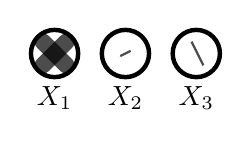
\begin{tikzpicture}[scale = .3]
      \draw[ultra thick] (0,0) circle (1cm);
      \draw[ultra thick] (3,0) circle (1cm);
      \draw[ultra thick] (6,0) circle (1cm);
      \node[below] at (0,-1) {$X_1$};
      \node[below] at (3,-1) {$X_2$};
      \node[below] at (6,-1) {$X_3$};
      % Marking the circles carelessly
      \draw[black,line width=6pt,line cap=round,opacity=.7] (0.5,-0.5) -- (-0.5,0.5);
      %\draw[black!70!white,thick] (3.1,-0.3) -- (2.7,0.5);
      \draw[black!70!white,thick] (5.8,0.5) -- (6.3,-0.5);
      %\draw[black,thick,line width=6pt,line cap=round,opacity=.7] (5.5,-0.5) -- (6.5,0.5);
      \draw[black,thick,line width=6pt,line cap=round,opacity=.7] (0.5,0.5) -- (-0.5,-0.5);
      \draw[black,thick,line cap=round,opacity=.7] (3.2,0.1) -- (2.8,-0.1);
      %\draw[black,thick,line width=6pt,line cap=round,opacity=.7] (5.5,0.5) -- (5.5,-0.5);
    \end{tikzpicture}
  \end{center}
  Shading may be incomplete, and there may be errent marks.
  We can use a \link[neural network]{https://en.wikipedia.org/wiki/Neural_network} to help solve this problem.
  This might sound really complicated, but at the end of the day, a neural network is just a matrix.


  Since the marks are incomplete, we visualize the input as continuous
  random variables $X_1$, $X_2$, and $X_3$; where a value of $1$ for
  $X_i$ would represent ``completely shaded'' and a value of $0$ for
  $X_i$ would represent completely unshaded. We can express these random
  variables as a column vector $\vec{X}$. Moreover, we may write the
  ``answer'' of whether the pattern is shaded correctly, using a column
  vector $\vec{Y}$, with two entries, also random variables $Y_1$ and
  $Y_2$, where $Y_1$ is the probability that the circles are filled in
  correctly, and $Y_2$ is the probability they are not.
  \[
  \vec{X} = \begin{pmatrix} X_1 \\ X_2 \\ X_3 \end{pmatrix} \qquad \vec{Y} = \begin{pmatrix} Y_1 \\ Y_2 \end{pmatrix}
  \]
  A matrix $H$ represents the neural network, say
  \[
  H = \begin{pmatrix}
     0.375 & -0.125 & -0.125 \\
     0.125 & 0.625 & 0.625
  \end{pmatrix}
  \quad \text{and we find} \quad
  H\vec{X} =
  \begin{pmatrix}
    0.288 \\
    0.163
  \end{pmatrix}
  \]
  for some $X$.  Interpret this result and represent this matrix
  equation as a system of equations.
  \begin{explanation}
    Since vector
    \[
    \vec{Y} =
    \begin{pmatrix}
    \answer[given]{0.288} \\
    \answer[given]{0.163}
    \end{pmatrix}
    \]
    We see that the drawn pattern, represented by $X_1$, $X_2$, and
    $X_3$, is likely the
    \wordChoice{\choice[correct]{correct}\choice{incorrect}} pattern.
    Writing
    \[
    H\vec{X} =
  \begin{pmatrix}
    0.288 \\
    0.163
  \end{pmatrix}
  \]
  corresponds to the system of equations:
  \begin{align*}
    \left(\answer[given]{0.375}\right)X_1 +  \left(\answer[given]{-0.125}\right) X_2 + \left(\answer[given]{-0.125}\right) X_3 &= 0.288 \\
    \left(\answer[given]{0.125}\right)X_1 + \left(\answer[given]{0.625}\right) X_2+  \left(\answer[given]{0.625}\right)X_3 &= 0.163
  \end{align*}
  \end{explanation}
\end{example}



%% \begin{example}[Cryptography]
%%   A Caeser cypher
%% \end{example}


  Networks, not to be confused with \textit{neural} networks, have
  numerous applications.



\begin{example}[Networks]
  A network is composed of junctions and branches.  and each junction
  can be described by an equation by equating the branches going in to
  branches going out. That is input = output. For example,

\begin{center}
\begin{tikzpicture}[scale=2]
\begin{scope}[very thick,decoration={
    markings,
    mark=at position 0.5 with {\arrow{>}}}
    ] 
\tikzset{vertex/.style = {shape=circle,draw,minimum size=1.5em}}
% vertices
\node[vertex] (a) at  (-1,1.7) {$A$};
\node[vertex] (b) at  (1,1.7) {$B$};
\node[vertex] (c) at  (0,0) {$C$};
%edges
\draw[postaction={decorate}] (a) to[bend right] (c);
\draw[postaction={decorate}] (c) to[bend right] (b);
\draw[postaction={decorate}] (b) to[bend right] (a);


\draw[postaction={decorate}] (a) to[bend left] (c);
\draw[postaction={decorate}] (a) to[bend right] (b);
\draw[postaction={decorate}] (b) to[bend right] (c);
\end{scope}
\end{tikzpicture}
\end{center}

gives:
\begin{eqnarray*}
20 &=& x_{1} + 2x_{2} + 30\\
x_{1} + 40 &=& x_{3}\\
2x_{2} + x_{3} + 30 &=& 40
\end{eqnarray*}
leading to:
\begin{eqnarray*}
x_{1}+2x_{2} &=& -10\\
x_{1} -x_{3}&=& -40\\
2x_{2} + x_{3}  &=& 10
\end{eqnarray*}
with augmented matrix:
\[\left(\begin{array}{ccc|c}
1 & 2 & 0 & -10\\
1 & 0 & -1 & -40\\
1 & 2 & 1 & 10
\end{array}\right)\]
\end{example}













\section{Multiplying matrices}



Matrix multiplication may seem strange at first. In fact, only certain
matrices can be multiplied together. As a general rule, we can only
multiply a $m \times n$ matrix by a $k \times \l$ matrix matrix if
$n=k$. That is if \textbf{the middle two numbers match}:
\[
\begin{matrix}
\begin{pmatrix}
    \bullet & \bullet & \bullet & \bullet & \bullet\\
    \bullet & \bullet & \bullet & \bullet & \bullet\\
\end{pmatrix}
&
\begin{pmatrix}
    \bullet & \bullet &\bullet \\\bullet & \bullet & \bullet \\  \bullet & \bullet & \bullet \\\bullet & \bullet & \bullet \\ \bullet & \bullet & \bullet \end{pmatrix} &= &
\begin{pmatrix}
  \bullet & \bullet &\bullet \\\bullet & \bullet &  \bullet
\end{pmatrix}\\
\begin{pmatrix}
  m\times n\\
  \text{matrix}
\end{pmatrix} &
\begin{pmatrix}
  n\times \l\\
  \text{matrix}
\end{pmatrix}
&= & \begin{pmatrix}
  m\times \l\\
  \text{matrix}
\end{pmatrix}
\end{matrix}
\]
The product then turns out to be a matrix of size $m\times \ell$, \textbf{the
outside numbers}.

\begin{question}
  Given three matrices
  \[
  A =\begin{pmatrix}
1 & -2 & 3 \\
0 & 5 & -6 \\
-7 & 8 & 0
\end{pmatrix},\quad B =\begin{pmatrix}
1 & 0 \\
-3 & 4 \\
5 & -6
\end{pmatrix}, \quad C =\begin{pmatrix}
0 & -2 & 3 \\
4 & 0 & -6
\end{pmatrix}\quad
  \]
  which of the following make sense?
  \begin{selectAll}\pdfOnly{\begin{multicols}{3}}
    \choice[correct]{$AA$}
    \choice[correct]{$AB$}
    \choice{$AC$}
    \choice{$BA$}
    \choice{$BB$}
    \choice[correct]{$BC$}
    \choice[correct]{$CA$}
    \choice[correct]{$CB$}
    \choice{$CC$}
    \pdfOnly{\end{multicols}}
  \end{selectAll}
  \begin{question}
    What are the dimensions of the products?
    \pdfOnly{\begin{multicols}{3}}
    \begin{enumerate}
    \item $AA$\begin{prompt}~is a $\answer{3}\times\answer{3}$ matrix.\end{prompt}
    \item $AB$\begin{prompt}~is a $\answer{3}\times\answer{2}$ matrix.\end{prompt}
    \item $BC$\begin{prompt}~is a $\answer{3}\times\answer{3}$ matrix.\end{prompt}
    \item $CA$\begin{prompt}~is a $\answer{2}\times\answer{3}$ matrix.\end{prompt}
    \item $CB$\begin{prompt}~is a $\answer{2}\times\answer{2}$ matrix.\end{prompt}
    \item $ABC$\begin{prompt}~is a $\answer{2}\times\answer{2}$ matrix.\end{prompt}
    \end{enumerate}
    \pdfOnly{\end{multicols}}
  \end{question}
\end{question}


%% We'll give several different explanations and interpretations of this
%% computation.

%% \subsection{As an extension of the dot product}
We can extend the concept of the dot product to explain how to
multiply a matrix by another matrix. Here is an example:
\begin{align*}AB &= \begin{pmatrix}
a_{1,1} & a_{1,2}\\
a_{2,1} & a_{2,2}
\end{pmatrix}
\begin{pmatrix}
b_{1,1} & b_{1,2}\\
b_{2,1} & b_{2,2}
\end{pmatrix}\\
&= \begin{pmatrix}
\row_1(A)^\transpose \dotp\col_1(B) & \row_1(A)^\transpose\dotp\col_2(B)\\
\row_2(A)^\transpose \dotp\col_1(B) & \row_2(A)^\transpose\dotp\col_2(B)
\end{pmatrix}\\
&= \begin{pmatrix}
a_{1,1}b_{1,1} + a_{1,2}b_{2,1} & a_{1,1}b_{1,2}+ a_{1,2}b_{2,2}\\
a_{2,1}b_{1,1} + a_{2,2}b_{2,1} & a_{2,1}b_{1,2} + a_{2,2}b_{2,2}
\end{pmatrix}
\end{align*}
We attempt to describe the structure of this product in the diagram below:
\begin{center}
\begin{tikzpicture}[]
     \matrix (matA) [%
       matrix of nodes,
       left delimiter={(},right delimiter={)}
     ] 
      {%
        \phantom{$\bullet$} & \phantom{$\bullet$} & \phantom{$\bullet$} & \phantom{$\bullet$} & \phantom{$\bullet$}\\
        \phantom{$\bullet$} & \phantom{$\bullet$} & \phantom{$\bullet$} & \phantom{$\bullet$} & \phantom{$\bullet$}\\
      };
      \draw[black,ultra thick,line cap=round] (matA-1-1.west)  -- (matA-1-5.east);
      \draw[black,ultra thick,line cap=round] (matA-2-1.west) -- (matA-2-5.east);
      
      \matrix (matB) [%
        matrix of nodes,right= of matA,
       left delimiter={(},right delimiter={)}
     ]
      {%
        \phantom{$\bullet$} & \phantom{$\bullet$} &\phantom{$\bullet$} \\\phantom{$\bullet$} & \phantom{$\bullet$} & \phantom{$\bullet$} \\  \phantom{$\bullet$} & \phantom{$\bullet$} & \phantom{$\bullet$} \\\phantom{$\bullet$} & \phantom{$\bullet$} & \phantom{$\bullet$} \\ \phantom{$\bullet$} & \phantom{$\bullet$} & \phantom{$\bullet$} \\
      };
      \draw[black,ultra thick,line cap=round] (matB-1-1.north)  -- (matB-5-1.south);
      \draw[black,ultra thick,line cap=round] (matB-1-2.north) -- (matB-5-2.south);
      \draw[black,ultra thick,line cap=round] (matB-1-3.north) -- (matB-5-3.south);
      
      \node[right=2ex of matB] {$=\begin{pmatrix}
  \boldsymbol{-}^\transpose\dotp\boldsymbol{|} & \boldsymbol{-}^\transpose\dotp\boldsymbol{|} &\boldsymbol{-}^\transpose\dotp\boldsymbol{|} \\\boldsymbol{-}^\transpose\dotp\boldsymbol{|} & \boldsymbol{-}^\transpose\dotp\boldsymbol{|} &  \boldsymbol{-}^\transpose\dotp\boldsymbol{|}
\end{pmatrix}$};
\end{tikzpicture}
\end{center}
Above the strange symbols
``$\boldsymbol{-}^\transpose\dotp\boldsymbol{|}$'' are supposed to
represent the transpose of the rows of $A$ being dotted with the
columns of $B$. Quite generally, if $A$ is an $m\times n$ matrix and $B$ is a $n\times
\l$ matrix, and $C = AB$ is a $m\times \l$ matrix, then
\[
C_{i,j} = \row_i(A)^\transpose\dotp \col_j(B).
\]
\begin{question} If
  \[
  A = \begin{pmatrix}
1 & -2 & 3 & 0 & -1 \\
4 & 0 & -5 & 6 & -7
  \end{pmatrix}\quad\text{and}\quad
  B=
  \begin{pmatrix}
1 & -2 & 3 \\
0 & 5 & -6 \\
-7 & 8 & 0 \\
4 & -5 & 6 \\
-1 & 2 & 1
\end{pmatrix}
  \]
  and $C = AB$, what is $C_{2,3}$?
  \begin{prompt}
    \[
    C_{2,3} = \answer{41}
    \]
  \end{prompt}
\end{question}







%% \subsection{Columns of the product}



%% Another viewpoint is to build the product as columns.  
%% \begin{align*}AB &= \begin{pmatrix}
%% a_{1,1} & a_{1,2}\\
%% a_{2,1} & a_{2,2}
%% \end{pmatrix}
%% \begin{pmatrix}
%% b_{1,1} & b_{1,2}\\
%% b_{2,1} & b_{2,2}
%% \end{pmatrix}\\
%% &= \begin{pmatrix}
%% \col_1(A)b_{1,1} + \col_2(A) b_{2,1} & \col_1(A)b_{1,2} + \col_2(A) b_{2,2}
%% \end{pmatrix}\\
%% &= \begin{pmatrix}
%% \begin{pmatrix}a_{1,1} \\ a_{2,1}\end{pmatrix}b_{1,1} + \begin{pmatrix}a_{1,2} \\ a_{2,2}\end{pmatrix}b_{2,1} & \begin{pmatrix}a_{1,1} \\ a_{2,1}\end{pmatrix}b_{1,2} + \begin{pmatrix}a_{1,2} \\ a_{2,2}\end{pmatrix}b_{2,2}
%% \end{pmatrix}\\
%% &= \begin{pmatrix}
%% a_{1,1}b_{1,1} + a_{1,2}b_{2,1} & a_{1,1}b_{1,2}+ a_{1,2}b_{2,2}\\
%% a_{2,1}b_{1,1} + a_{2,2}b_{2,1} & a_{2,1}b_{1,2} + a_{2,2}b_{2,2}
%% \end{pmatrix}
%% \end{align*}

%% We attempt to describe the structure of this product in the diagram below:
%% \begin{center}
%% \begin{tikzpicture}[]
%%      \matrix (matA) [%
%%        matrix of nodes,
%%        left delimiter={(},right delimiter={)}
%%      ] 
%%       {%
%%         \phantom{$\bullet$} & \phantom{$\bullet$} & \phantom{$\bullet$} & \phantom{$\bullet$} & \phantom{$\bullet$}\\
%%         \phantom{$\bullet$} & \phantom{$\bullet$} & \phantom{$\bullet$} & \phantom{$\bullet$} & \phantom{$\bullet$}\\
%%       };
%%       \draw[black,ultra thick,line cap=round] (matA-1-1.north)  -- (matA-2-1.south);
%%       \draw[black,ultra thick,line cap=round] (matA-1-2.north)  -- (matA-2-2.south);
%%       \draw[black,ultra thick,line cap=round] (matA-1-3.north)  -- (matA-2-3.south);
%%       \draw[black,ultra thick,line cap=round] (matA-1-4.north)  -- (matA-2-4.south);
%%       \draw[black,ultra thick,line cap=round] (matA-1-5.north)  -- (matA-2-5.south);
      
%%       \matrix (matB) [%
%%         matrix of nodes,right=of matA,
%%        left delimiter={(},right delimiter={)}
%%      ]
%%       {%
%%         $\bullet$ & $\bullet$ &$\bullet$ \\$\bullet$ & $\bullet$ & $\bullet$ \\  $\bullet$ & $\bullet$ & $\bullet$ \\$\bullet$ & $\bullet$ & $\bullet$ \\ $\bullet$ & $\bullet$ & $\bullet$ \\
%%       };
%%       \draw[black!20!white,line width=1ex,line cap=round] (matB-1-1.north)  -- (matB-5-1.south);
%%       \draw[black!20!white,ultra thick,line width=1ex,line cap=round] (matB-1-2.north) -- (matB-5-2.south);
%%       \draw[black!20!white,ultra thick,line width=1ex,line cap=round] (matB-1-3.north) -- (matB-5-3.south);
      
%%       \node[right=2ex of matB] {$=\begin{pmatrix}
%%   \boldsymbol{\Big|\mkern-4mu\cdot\mkern-4mu\Big|\mkern-4mu\cdot\mkern-4mu\Big|\mkern-4mu\cdot\mkern-4mu\Big|\mkern-4mu\cdot\mkern-4mu\Big|\cdot} & \boldsymbol{\Big|\mkern-4mu\cdot\mkern-4mu\Big|\mkern-4mu\cdot\mkern-4mu\Big|\mkern-4mu\cdot\mkern-4mu\Big|\mkern-4mu\cdot\mkern-4mu\Big|\cdot} & \boldsymbol{\Big|\mkern-4mu\cdot\mkern-4mu\Big|\mkern-4mu\cdot\mkern-4mu\Big|\mkern-4mu\cdot\mkern-4mu\Big|\mkern-4mu\cdot\mkern-4mu\Big|\cdot} \\
%%         \end{pmatrix}$};
%%       \matrix (matBp) [%
%%         matrix of nodes,right=of matA,
%%        left delimiter={(},right delimiter={)}
%%      ]
%%       {%
%%         $\bullet$ & $\bullet$ &$\bullet$ \\$\bullet$ & $\bullet$ & $\bullet$ \\  $\bullet$ & $\bullet$ & $\bullet$ \\$\bullet$ & $\bullet$ & $\bullet$ \\ $\bullet$ & $\bullet$ & $\bullet$ \\
%%       };
%% \end{tikzpicture}
%% \end{center}
%% Above the strange symbols
%% ``$\boldsymbol{\Big|\mkern-4mu\cdot\mkern-4mu\Big|\mkern-4mu\cdot\mkern-4mu\Big|\mkern-4mu\cdot\mkern-4mu\Big|\mkern-4mu\cdot\mkern-4mu\Big|\cdot}$''
%% are supposed to represent the sum of the columns of $A$ each multipled
%% by an element of a column of $B$.  Quite generally, if $A$ is an
%% $m\times n$ matrix and $B$ is a $n\times \l$ matrix, and $C = AB$ is a
%% $m\times \l$ matrix, then
%% \[
%% \col_i(C) = \sum_{k=1}^n \col_k(A)b_{k,i}
%% \]
%% that is,
%% \begin{align*}
%%   C &= \begin{pmatrix} \col_1(C) & \col_2 (C) & \cdots & \col_{\l}(C) \end{pmatrix}\\
%%   &=  \begin{pmatrix} \sum_{k=1}^n \col_k(A)b_{k,1} & \sum_{k=1}^n \col_k(A)b_{k,2} & \cdots & \sum_{k=1}^n \col_k(A)b_{k,\l}\end{pmatrix}
%% \end{align*}
%% \begin{question} If
%%   \[
%%   A = \begin{pmatrix}
%% 1 & -2 & 3 & 0 & -1 \\
%% 4 & 0 & -5 & 6 & -7
%%   \end{pmatrix}\quad\text{and}\quad
%%   B=
%%   \begin{pmatrix}
%% 1 & -2 & 3 \\
%% 0 & 5 & -6 \\
%% -7 & 8 & 0 \\
%% 4 & -5 & 6 \\
%% -1 & 2 & 1
%% \end{pmatrix}
%%   \]
%%   and $C = AB$, what is $\col_2(C)$?
%%   %\begin{prompt}
%%     \[
%%     \col_2(C) =  \col_1(A)b_{1,2} +  \col_2(A)b_{2,2}+  \col_3(A)b_{3,2} + \col_4(A) b_{4,2} + \col_5(A) b_{5,2}
%%     \]
%%   %\end{prompt}
%% \end{question}











%% \subsection{Rows of the product}


%% \begin{align*}AB &= \begin{pmatrix}
%% a_{1,1} & a_{1,2}\\
%% a_{2,1} & a_{2,2}
%% \end{pmatrix}
%% \begin{pmatrix}
%% b_{1,1} & b_{1,2}\\
%% b_{2,1} & b_{2,2}
%% \end{pmatrix}\\
%% &= \begin{pmatrix}
%% a_{1,1}\row_1(B) + a_{1,2}\row_2(B) \\ a_{2,1}\row_1(B) +  a_{2,2}\row_2(B)
%% \end{pmatrix}\\
%% &= \begin{pmatrix}
%% a_{1,1}\begin{pmatrix} b_{1,1} & b_{1,2}\end{pmatrix} + a_{1,2}\begin{pmatrix} b_{2,1} & b_{2,2}\end{pmatrix} \\ a_{2,1}\begin{pmatrix} b_{1,1} & b_{1,2}\end{pmatrix} +  a_{2,2}\begin{pmatrix} b_{2,1} & b_{2,2}\end{pmatrix}
%% \end{pmatrix}\\
%% &= \begin{pmatrix}
%% a_{1,1}b_{1,1} + a_{1,2}b_{2,1} & a_{1,1}b_{1,2}+ a_{1,2}b_{2,2}\\
%% a_{2,1}b_{1,1} + a_{2,2}b_{2,1} & a_{2,1}b_{1,2} + a_{2,2}b_{2,2}
%% \end{pmatrix}
%% \end{align*}

%% Quite generally, if $A$ is an $m\times n$ matrix and $B$ is a $n\times
%% \l$ matrix, and $C = AB$ is a $m\times \l$ matrix, then
%% \[
%% \row_i(C) = \sum_{k=1}^n a_{i,k}\row_k(B)
%% \]
%% that is,
%% \[
%%   C = \begin{pmatrix} \row_1(C) \\ \row_2 (C) \\ \vdots \\ \row_{m}(C) \end{pmatrix}
%%   =  \begin{pmatrix} \sum_{k=1}^n a_{1,k}\row_k(B) \\ \sum_{k=1}^n a_{2,k}\row_k(B) \\ \vdots \\ \sum_{k=1}^n a_{m,k}\row_k(B)\end{pmatrix}
%% \]















\begin{question}
For the following matrices, find $AB$ and $BA$.
\[
A= \left(\begin{array}{cc}
5 & 0 \\
2 & 1
\end{array}\right), \hspace{.5cm} B = \left(\begin{array}{cc}
3 & -1 \\
2 & 0
\end{array}\right)
\]
\begin{prompt}
\[
AB = \left(\begin{array}{cc}
\answer[given]{15} & \answer[given]{-5}\\
\answer[given]{8} & \answer[given]{-2}
\end{array}\right)\]

\[BA = \left(\begin{array}{cc}
\answer[given]{13} & \answer[given]{-1}\\
\answer[given]{10} & \answer[given]{0}
\end{array}\right)\]
\end{prompt}
Do the two multiplications give the same result?
\begin{prompt}
  \begin{multipleChoice}
    \choice{Yes.}
    \choice[correct]{No.}
  \end{multipleChoice}
\end{prompt}
\end{question}




For example,
\[\left(\begin{array}{ccc}
1 & -1 & 0\\
2 & 0 & 4 \\
5 & 3 & 1
\end{array}\right) \left(\begin{array}{ccc}
5 & 1 & 0\\
-1 & -2 & 0\\
1 & 0 & 2
\end{array}\right)\]
\[= \left(\begin{array}{ccc}
(1)(5) + (-1)(-1)+ (0)(1) & 1 + 2+ 0 & 0 + 0+ 0\\
10 + 0 + 4 & 2 + 0+0 & 0 + 0+8\\
25+ (-3) + 1 & 5 + -6+0 & 0 + 0+ 2
\end{array}\right)\]
\[= \left(\begin{array}{ccc}
6 & 3 & 0\\
14& 2 & 8\\
23 & -1 & 2
\end{array}\right)
\]
It is helpful to first write the sum since there might be many small calculations and easy to make mistakes. It is important to write the matrices neatly and put enough space between entries.






\section{Matrices transform data}


\begin{example}[Financial Transactions]
  Recall that a bookstore sells a variety of books with each type of
  book sold in one month stored as a row vector
  \[
  \vec{s} = \begin{pmatrix}141 & 304 & 249 & 199 & 251 \end{pmatrix}
  \]
  with the entries representing the categories: Science Fiction,
  Fantasy, Mystery, Romance, Historical in that order.  Suppose last
  month the book store bought $200$ Science Fiction, $400$ Fantasy, $300$
  Mystery, $250$ Romance, $300$ Historical books. What percentage of each
  category was sold this month?
  \begin{explanation}
    Let
    \[
    T =
    \begin{pmatrix}
      100/200 & 0 &    0   &   0    &   0 \\
      0 & 100/400 &    0   &   0    &   0 \\
      0 &   0   &  100/300 &   0    &   0 \\
      0 &   0   &    0   & 100/250  &   0 \\
      0 &   0   &    0   &   0    & 100/300
    \end{pmatrix}
    \]
    Each entry of the matrix $T$ is of the form:
    \[
    100 \cdot \frac{1}{(\text{Stock})}
    \]
    where $(\text{Stock})$ represents the number of books the
    bookstore bought to sell.  We can solve our problem by computing
    \[
    \vec{s} T =
    \]
    So we see
  \end{explanation}

\end{example}




\begin{example}[Navigation]
  Scale/normalize fincinal data etc.
\end{example}
























































\section{Types of matrices}
Earlier, we introduced the transpose of a vector:
\[
\vec{u} = \left(\begin{array}{ccc}
1 & -1 & 0
\end{array}\right)
\hspace{.4cm}\Rightarrow\hspace{.4cm}
\vec{u}^{\transpose} = \begin{pmatrix}
1\\
-1\\
0
\end{pmatrix}
\]
So transpose switched a $\left(1\times 3\right)$- matrix to a $\left(3\times 1\right)$- matrix. The same concept applies to any larger matrix. The transpose operation switches all the rows to columns:
\[
A = \left(\begin{array}{ccc}
2 & -1 & 0\\
-3 & 4 & 5\\
1 & -2 & 0
\end{array}\right)
\hspace{.4cm}\Rightarrow\hspace{.4cm}
A^{\transpose} = \left(\begin{array}{ccc}
2 & -3 & 1\\
-1 & 4 & -2\\
0& 5 & 0
\end{array}\right)
\]
Thus, the first row of $A$ becomes the first column of $A^{\transpose}$ and the second row of $A$ becomes the second column of $A^{\transpose}$ and so forth.
\begin{question}
If
\[A= \left(\begin{array}{ccc}
-3 & 0 & 1\\
5 & 8 & 10
\end{array}\right), \hspace{.5cm} B = \left(\begin{array}{ccc}
7 & -2 & -1 \\
0 & 1 & 9 \\
5 & 4 & 2
\end{array}\right)\]
Find $A^{\transpose}$ and $B^{\transpose}$.

\begin{prompt}
\[A^{T} = \left(\begin{array}{cc}
\answer[given]{-3} & \answer[given]{5}\\
\answer[given]{0} & \answer[given]{8}\\
\answer[given]{1} & \answer[given]{10}
\end{array}\right), \hspace{.5cm} B^{\transpose}= \left(\begin{array}{ccc}
\answer[given]{7} & \answer[given]{0} & \answer[given]{5}\\
\answer[given]{-2} & \answer[given]{1} & \answer[given]{4}\\
\answer[given]{-1} & \answer[given]{9} & \answer[given]{2}
\end{array}\right)\]
\end{prompt}
\end{question}

\begin{question}
If
\[
A= \left(\begin{array}{ccc}
-3 & 0 & 1\\
4 & 0 & 2\\
-1 & 5 & 0
\end{array}\right), \hspace{.5cm}
B = \left(\begin{array}{ccc}
1 & -1 & 0\\
0 & 2 & 1\\
-3 & 4 & 0
\end{array}\right)\]
Compute the following. \\

a. $2A^{\transpose}$ \begin{prompt} \[= \left(\begin{array}{ccc}
\answer[given]{-6} & \answer[given]{8}& \answer[given]{-2}\\
\answer[given]{0} & \answer[given]{0}& \answer[given]{10}\\
\answer[given]{2} & \answer[given]{4}& \answer[given]{0}
\end{array}\right)\]\end{prompt}\\

b. $AB^{\transpose}$ \begin{prompt} \[= \left(\begin{array}{ccc}
\answer[given]{-3} & \answer[given]{1}& \answer[given]{9}\\
\answer[given]{4} & \answer[given]{2}& \answer[given]{-12}\\
\answer[given]{-6} & \answer[given]{10}& \answer[given]{23}
\end{array}\right)\]\end{prompt}\\

c. $A^{\transpose} + AB$ \begin{prompt} \[=\left(\begin{array}{ccc}
\answer[given]{-9} & \answer[given]{11}& \answer[given]{-1}\\
\answer[given]{-2} & \answer[given]{4}& \answer[given]{5}\\
\answer[given]{0} & \answer[given]{13}& \answer[given]{5}
\end{array}\right)\]\end{prompt}
\end{question}

As in vectors, for any matrices $A$ and $B$, $\left(A^{\transpose}\right)^{\transpose} = A$ and $\left(A+ B\right)^{\transpose} = A^{\transpose} + B^{\transpose}$. Another property of transpose operation which is often used is
\[
\left(AB\right)^{\transpose} = B^{\transpose} A^{\transpose}
\]
Thus, their order changes after taking the transpose of each.
\begin{question}
Let
\[
A= \left(\begin{array}{cc}
2 & -1 \\
3 & 4
\end{array}\right), \hspace{.5cm} B = \left(\begin{array}{cc}
7 & 5 \\
0 & 1
\end{array}\right)
\]
Find $\left(AB\right)^{\transpose}$ and compare it with $B^{\transpose}A^{\transpose}$.

\begin{prompt}
\[
AB = \left(\begin{array}{cc}
\answer[given]{14} & \answer[given]{9}\\
\answer[given]{21} & \answer[given]{19}
\end{array}\right)
\hspace{.4cm} \Rightarrow \hspace{.4cm}
\left(AB\right)^{\transpose} = \left(\begin{array}{cc}
\answer[given]{14} & \answer[given]{21}\\
\answer[given]{9} & \answer[given]{19}
\end{array}\right)
\]
\[
A^{\transpose}= \left(\begin{array}{cc}
\answer[given]{2} & \answer[given]{3}\\
\answer[given]{-1} & \answer[given]{4}
\end{array}\right), \hspace{.5cm}
B^{\transpose} = \left(\begin{array}{cc}
\answer[given]{7} & \answer[given]{0}\\
\answer[given]{5} & \answer[given]{1}
\end{array}\right)
\hspace{.4cm} \Rightarrow \hspace{.4cm}
B^{\transpose} A^{\transpose}  = \left(\begin{array}{cc}
\answer[given]{14} & \answer[given]{21}\\
\answer[given]{9} & \answer[given]{19}
\end{array}\right)
\]
\end{prompt}
\end{question}








\begin{proposition}[Transpose matrix multiplication]
  Suppose we have a $m\times n$ matrix $A$ and an $n\times \l$ matrix $B$. In this case:
  \[
  (BA)^\transpose = A^\transpose B^\transpose
  \]
  \begin{explanation}
    Using the dot product interpretation of matrix multiplication, we can write
    \[
      (BA)_{i,j} = \row_i(B)^\transpose \dotp \col_j(A)
    \]
    Now, write with me (you have to write along to really understand)
    \begin{align*}
      (BA)_{i,j}^\transpose &= \row_j(B)^\transpose \dotp \col_i(A) & & (\text{transpose swaps $i$ and $j$})\\
      &= \col_j(B^\transpose)^\transpose \dotp \row_i(A^\transpose) & & (\text{transpose swaps rows and columns})\\
      &= \row_i(A^\transpose)^\transpose \dotp \col_j(B^\transpose) & & (\vec x^\transpose \dotp \vec y = \vec x\dotp \vec y^\transpose)\\
      &= A^\transpose B^\transpose.
    \end{align*}
  \end{explanation}
\end{proposition}
















Let us explore some types of matrices that usually are used in linear
algebra. The zero matrix, usually denoted as $\textbf{O}_{m \times n}$ is
an $m \times n$ matrix with each of its entries being zero. For example,
\[
\textbf{O}_{2\times 3} = \left(\begin{array}{ccc}
0 & 0 &0 \\
0 & 0 & 0
\end{array}\right), \hspace{.5cm} \textbf{O}_{4\times 2} = \left(\begin{array}{cc}
0 & 0 \\
0 & 0 \\
0 & 0\\
0 & 0
\end{array}\right)\]
It is not hard to see that the zero matrix multiplied by a matrix gives a zero matrix:
\[
\left(\begin{array}{ccc}
2 & -1 & 0 \\
3 & 4 & 3\\
1 & -2 & 7
\end{array}\right) \left(\begin{array}{ccc}
0 &0 &0 \\
0 &0 &0 \\
0 &0 &0
\end{array}\right) = \left(\begin{array}{ccc}
0 &0 &0 \\
0 &0 &0 \\
0 &0 &0
\end{array}\right)
\]
and $\textbf{O}_{3\times 3} A = \textbf{O}_{3 \times 3}$.


Another important type of matrix is the identity matrix, denoted as
$I_{m \times n}$. It is a matrix whose diagonal entries are $1$ and its
every other entry is zero. In particular, when $m = n$,
$I_{n \times n}$ is often denoted simply as $I_n$, and this square matrix
is called the \dfn{identity matrix}. For example,
\[
  I_{2\times 2}=
  \left(\begin{array}{cc}
    1 & 0 \\
    0 & 1
  \end{array}\right), \hspace{.5cm}  I_{4\times 4} = \left(\begin{array}{cccc}
    1 & 0 & 0 & 0 \\
    0 & 1 & 0& 0 \\
    0& 0 & 1 & 0\\
    0 & 0 & 0 & 1
  \end{array}\right)
\]
% Note that the identity matrix is a square matrix ( has the same number
% of rows as columns).
The fundamental property of the identity matrix is that it acts as $1$
as in regular multiplication. That is, $AI = A$ and $IA= A$. For
example, one can check that
\[
\left(\begin{array}{cc}
a_{1} & a_{2}\\
a_{3} & a_{4}
\end{array}\right) \left(\begin{array}{cc}
1 & 0\\
0 &1
\end{array}\right) = \left(\begin{array}{cc}
a_{1} & a_{2}\\
a_{3} & a_{4}
\end{array}\right)
\]
and
\[\left(\begin{array}{cc}
1 & 0\\
0 &1
\end{array}\right)\left(\begin{array}{cc}
a_{1} & a_{2}\\
a_{3} & a_{4}
\end{array}\right)= \left(\begin{array}{cc}
a_{1} & a_{2}\\
a_{3} & a_{4}
\end{array}\right) \]

\begin{question}
Write down the $3 \times 3$ identity matrix and show that $AI = IA = A$ for
\[A =  \left(\begin{array}{ccc}
2 & 3 & 4\\
0  & 1 & -1\\
5 & 7 & 9
\end{array}\right)
\]

\begin{prompt}
\[
I_{3\times 3} = \left(\begin{array}{ccc}
\answer[given]{1} & \answer[given]{0} & \answer[given]{0}\\
\answer[given]{0} & \answer[given]{1} & \answer[given]{0}\\
\answer[given]{0} & \answer[given]{0} & \answer[given]{1}
\end{array}\right)
\]
Then,
\[
AI = \left(\begin{array}{ccc}
2 & 3 & 4\\
0  & 1 & -1\\
5 & 7 & 9
\end{array}\right)\left(\begin{array}{ccc}
\answer[given]{1} & \answer[given]{0} & \answer[given]{0}\\
\answer[given]{0} & \answer[given]{1} & \answer[given]{0}\\
\answer[given]{0} & \answer[given]{0} & \answer[given]{1}
\end{array}\right)= \left(\begin{array}{ccc}
\answer[given]{2} & \answer[given]{3} & \answer[given]{4}\\
\answer[given]{0} & \answer[given]{1} & \answer[given]{-1}\\
\answer[given]{5} & \answer[given]{7} & \answer[given]{9}
\end{array}\right)\]
and
\[
IA = \left(\begin{array}{ccc}
\answer[given]{1} & \answer[given]{0} & \answer[given]{0}\\
\answer[given]{0} & \answer[given]{1} & \answer[given]{0}\\
\answer[given]{0} & \answer[given]{0} & \answer[given]{1}
\end{array}\right)\left(\begin{array}{ccc}
2 & 3 & 4\\
0  & 1 & -1\\
5 & 7 & 9
\end{array}\right)= \left(\begin{array}{ccc}
\answer[given]{2} & \answer[given]{3} & \answer[given]{4}\\
\answer[given]{0} & \answer[given]{1} & \answer[given]{-1}\\
\answer[given]{5} & \answer[given]{7} & \answer[given]{9}
\end{array}\right)\]
\end{prompt}
\end{question}


Yet another useful type of matrix is the matrix of all ones which is
often denoted by $J_{m \times n}$. For example,
\[
  J_{3} = J_{3 \times 3} =
  \begin{pmatrix}
    1 & 1 & 1 \\
    1 & 1 & 1 \\
    1 & 1 & 1
  \end{pmatrix}, \qquad
  J_{4 \times 2} =
  \begin{pmatrix}
    1 & 1 \\
    1 & 1 \\
    1 & 1 \\
    1 & 1
  \end{pmatrix}, \qquad
  J_{5 \times 1} = \vec{1}_5 =
  \begin{pmatrix}
    1 \\ 1 \\ 1 \\ 1 \\ 1 \\
  \end{pmatrix}.
\]
Recall that we have already introduced the notation $\vec{1}$ for the
column vector of all ones in the data analysis example. This can be
thought of as a special type of all-ones matrix that has only one
column.

Even though $J$ does not satisfy neat algebraic properties such as
$A \vec{O} = \vec{O}$ or $AI = IA = A$, this all-ones matrix arises in
many fields of applications such as graph theory and statistics.

\begin{remark}[Computational notes]
  The three types of matrices introduced above are very commonly used
  in applications, so many numerical programming languages offer
  utilities that generate these matrices with ease. For instance, in
  MATLAB, each of $\vec{O}_{m \times n}$, $J_{m \times n}$, and $I_{m \times n}$ can be
  constructed in one line of code:
\begin{verbatim}
  >> zeros(m, n)
  >> ones(m, n)
  >> eye(m, n)
\end{verbatim}
\end{remark}

\begin{example}[Data Analysis (revisited) -- Computing Variances]
  This is continuation of the data analysis example in which we
  formulated the average of a single student's homework scores using a
  dot product.

  In this example, we now consider a slightly different situation in
  which we analyze the final exam scores of the entire linear algebra
  class. This class is very popular among STEM majors and has 200
  students in it. Furthermore, due to privacy reasons, we will encrypt
  the exam scores in a column vector $\vec{x}$ of with $n=200$
  entries, written abstractly as
  \[
    \vec{x} =
    \begin{pmatrix}
      x_1 \\ x_2 \\ \vdots \\ x_n
    \end{pmatrix}
    \qquad
    \begin{array}{l}
      \text{Student $1$}\\
      \text{Student $2$}\\
      \vdots \\
      \text{Student $n$}
    \end{array}
  \]
  instead of writing out all 200 scores. Let $\vec{1} = J_{n \times 1}$ be
  the column vector of all ones.

  \begin{enumerate}
  \item The average final exam score $\mu$ of the entire class is given
    by
    \begin{equation*}
      \mu = \frac{1}{n} \vec{1}^\transpose \vec{x}.
    \end{equation*}
    This was explained previously.
  \item The deviations from the average, $x_1 - \mu$, $x_2 - \mu$, \ldots, $x_n
    - \mu$, can be packaged into a column vector, say $\overline{\vec{x}}$,
    by
    \begin{align*}
      \overline{\vec{x}}
      & =
        \begin{pmatrix}
          x_1 - \mu \\ x_2 - \mu \\ \vdots \\ x_n - \mu
        \end{pmatrix} \\
      & =
        \begin{pmatrix}
        x_1 \\ x_2 \\ \vdots \\ x_n
        \end{pmatrix}
        - \mu
        \begin{pmatrix}
          1 \\ 1 \\ \vdots \\ 1
        \end{pmatrix} \\
      & = \vec{x} - \mu \vec{1}.
    \end{align*}
    Using the property of the identity matrix, we can write $\vec{x}$
    as $I \vec{x}$. Furthermore, since $\mu \vec{1} = \vec{1} \mu$, we can
    write simplify the last line as
    \begin{align*}
      \overline{\vec{x}}
      & = I \vec{x} - \vec{1} \left( \frac{1}{n} \vec{1}^\transpose
        \vec{x} \right) \\
      & = \bigl( I - \frac{1}{n} \underbrace{\vec{1} \vec{1}^\transpose}_{=J} \bigr) \vec{x}.
      % & = \underbrace{\left( I - \frac{1}{n} \vec{1}
      %   \vec{1}^\transpose \right)}_{=H} \vec{x} = H \vec{x}.
    \end{align*}
    Note that the product $\vec{1} \vec{1}^\transpose$ is in the form
    of a row vector followed by a column vector, which results in a
    square matrix of all ones, that is, $J = J_{n}$. The upshot is
    that if we define a new matrix $H$ by
    \[
      H = I - \frac{1}{n} J =
      \begin{pmatrix}
        1-\frac{1}{n} & -1 & -1 & \cdots & -1 \\
        -1 & 1-\frac{1}{n} & -1 & \cdots & -1 \\
        -1 & -1 & 1-\frac{1}{n} & \cdots & -1 \\
        \vdots & \vdots & \vdots & \ddots & \vdots \\
        -1 & -1 & -1 & \cdots & 1-\frac{1}{n}
      \end{pmatrix},
    \]
    then the vector $\overline{\vec{x}}$ of deviations or centered
    data is obtained simply by the matrix-vector product
    \[
      \overline{\vec{x}} = H\vec{x}.
    \]
  \item The average of the squared deviations, commonly known as the
    variance and denoted by $\sigma^2$, of the final exam scores is
    computed by
    \begin{align*}
      \sigma^2
      & = \frac{1}{n} \sum_{i=1}^n \overline{x}_i^2 \\
      & = \frac{1}{n}
        \begin{pmatrix}
          \overline{x}_1 & \overline{x}_2 & \cdots & \overline{x}_n
        \end{pmatrix}
        \begin{pmatrix}
          \overline{x}_1 \\ \overline{x}_2 \\ \vdots \\ \overline{x}_n
        \end{pmatrix} \\
      & = \frac{1}{n} \overline{\vec{x}}^\transpose \overline{\vec{x}}.
    \end{align*}
    Note that the variance is a sum of squares and, by now, it is no
    surprise to us that it can be expressed as a dot product! In fact,
    we have already seen the dot product of the form
    $\overline{\vec{x}}^\transpose \overline{\vec{x}}$ in the
    definition of the Euclidean norm.

    One can go a step further and substitute
    $\overline{\vec{x}} = H \vec{x}$ in the last line to obtain
    \[
      \sigma^2
      = \frac{1}{n} \left( H \vec{x} \right)^\transpose \left( H
        \vec{x} \right)
      = \frac{1}{n} \vec{x}^\transpose \left( H^\transpose H \right) \vec{x}.
    \]
    The form $\vec{x}^\transpose \text{(square matrix)} \vec{x}$ in
    the last line is called the \textit{\link[quadratic
      form]{https://en.wikipedia.org/wiki/Quadratic_form}}. This
    mathematical structure provides a powerful framework across many
    branches of mathematics, not just linear algebra, and many fields
    of applications.
  \end{enumerate}
\end{example}




For some interesting extra reading check out:
\begin{itemize}
\item \link[\textit{Earliest Uses of Symbols for Matrices and Vectors},  MacTutor History of Mathematics, (University of St Andrews, Scotland, February 2000.]{https://mathshistory.st-andrews.ac.uk/Miller/mathsym/matrices/}
\end{itemize}



\end{document}
